\documentclass[a4paper, 11pt]{article}

\usepackage[text={17cm, 24cm}]{geometry}
\usepackage[czech]{babel}
\usepackage{amsmath}
\usepackage{minted}
\usepackage{xcolor}
\usepackage{sourcecodepro}
\usepackage{tabularx}
\usepackage{booktabs}
\usepackage{hyperref}
\usepackage{graphicx}
\usepackage{wrapfig}
\usepackage{titling}

\pretitle{\begin{center}\huge\bfseries}
\posttitle{\end{center}}

\renewcommand{\texttt}[1]{{\footnotesize\ttfamily #1}}

\newcolumntype{R}{>{\raggedleft\arraybackslash}X}
\newcolumntype{C}{>{\centering\arraybackslash}X}

\definecolor{codegreen}{rgb}{0,0.6,0}
\definecolor{codeblue}{rgb}{0,0,0.6}
\definecolor{codered}{rgb}{0.6,0,0}

\setminted{ 
    linenos=true,
    framesep=2mm, 
    xleftmargin=5mm, 
    xrightmargin=5mm, 
    tabsize=4, 
    fontsize=\footnotesize, 
    encoding=utf8,
    numbersep=5pt, 
    numbers=left,
    escapeinside=||
}

\title{MSP projekt 2 -- report}
\author{Ondřej Koumar, xkouma02}
\date{}

\begin{document}
\maketitle

\vspace{-3em}

\section{Věrohodnost}

Zvolená parametrizace Weibullova rozdělení je $f(x, k, \lambda)$, kde $k$ určuje tvar a~$\lambda$ určuje roztažení funkce hustoty. Ta je ve tvaru:
\[
    f(x, k, \lambda) = 
    \begin{cases}
        \frac{k}{\lambda} \left( \frac{x}{\lambda} \right)^{k-1} e^{\left( \frac{x}{\lambda} \right)^{k}}, & x\geq 0, \\
        0, & x < 0
    \end{cases}
\]

\subsection{Logaritmická věrohodnostní funkce a parciální derivace podle parametrů}
Věrohodnostní funkce pro $n$ pozorování Weibullova rozdělení má tvar:
\[
    L(k, \lambda) = \prod_{i=1}^{n} \left[ \frac{k}{\lambda} \cdot \left( \frac{x_{i}}{\lambda} \right)^{k-1} \cdot e^{\left( \frac{x_{i}}{\lambda}\right)^{k}} \right]
\]
Musíme ale počítat s~cenzorovanými daty.
Weibullovo rozdělení je definováno na intervalu $[0, \infty)$ a~je zobecněním exponenciálního rozdělení.
Někteří studenti přestali reagovat na zprávy po známé době a~stále pracovali v~oboru.
To jsou zprava cenzorovaná data, která musíme započítat do věrohodnostní funkce, což provedeme vynásobením součinu pravděpodobností, že po čase, kdy přestali reagovat, stále pracovali v~oboru.

Předpokládejme $m$ cenzorovaných a~$n$ necenzorovaných pokusů Weibullova rozdělení.
Vě\-ro\-hod\-nost\-ní funkce bude vypadat následovně:
\begin{align*}
    L(k, \lambda) &= \prod_{i=0}^{m}\left(1 - F(x_i)\right) \cdot \prod_{i=1}^{n} f(x_i) = \\
    &= \prod_{j=0}^{m} \left[1 - \left( 1 - e^{\left( -\frac{x_j}{\lambda} \right) ^k} \right) \right] \cdot \prod_{i=1}^{n} \left[ \frac{k}{\lambda} \cdot \left( \frac{x_{i}}{\lambda} \right)^{k-1} \cdot e^{\left( \frac{x_{i}}{\lambda}\right)^{k}} \right] = \\
    &= \prod_{j=0}^{m} \left[ e^{\left( -\frac{x_j}{\lambda} \right) ^k} \right] \cdot \prod_{i=1}^{n} \left[ \frac{k}{\lambda} \cdot \left( \frac{x_{i}}{\lambda} \right)^{k-1} \cdot e^{\left( \frac{x_{i}}{\lambda}\right)^{k}} \right] \\
\end{align*}


Po zlogaritmování věrohodnostní funkce dostaneme logaritmickou věrohodnostní funkci:
\begin{align*}   
    \ell(k, \lambda) &= \sum_{j=0}^{m}  \left( -\frac{x_j}{\lambda} \right)^k + \left[ \sum_{i=1}^{n} \left[ \ln \left( \frac{k}{\lambda} \right) \right] + \sum_{i=1}^{n} \left[ (k-1) \ln \left( \frac{x_{i}}{\lambda} \right) \right] - \sum_{i=1}^{n} \left[ \left( \frac{x_i}{\lambda} \right)^k \right] \right] = \\
    &= - \sum_{j=0}^{m} \left(\frac{x_j}{\lambda} \right)^k + n \cdot \ln(k) - n \cdot k \cdot \ln(\lambda) + (k-1) \cdot \sum_{i=1}^{n} \ln(x_i) - \sum_{i=1}^{n} \left[ \left( \frac{x_i}{\lambda} \right)^k \right]
\end{align*}

Parciální derivace $\ell(k, \lambda)$ podle parametru $k$:
\[
    \frac{\partial \ell(k, \lambda)}{\partial k} = - \sum_{j=0}^{m} \left[ \left( \frac{x_j}{\lambda} \right)^k \cdot \left( \frac{x_j}{\lambda} \right) \right] + \frac{n}{k} - n \cdot \ln(\lambda) + \sum_{i=0}^{n} \ln(x_i) - \sum_{i=0}^{n} \left[ \left( \frac{x_i}{\lambda} \right)^k \cdot \left( \frac{x_i}{\lambda} \right) \right]
\] 

Pro parciální derivaci $\ell(k, \lambda)$ podle parametru $\lambda$ si nejdříve vypočítejme derivaci prvního a~posledního členu:

\begin{align*}
    \frac{\partial \sum_{i=0}^{n} \left[ \left( \frac{x_i}{\lambda} \right)^k \right] }{\partial \lambda} &= \frac{\partial \sum_{i=1}^{n} \left[ {x_i}^k \cdot \lambda^{-k} \right]}{\partial \lambda} = \\
    &= \sum_{i=0}^{n} \left[ {x_i}^k \cdot (-k) \cdot \lambda^{-k-1} \right] = \\
    &= \sum_{i=0}^{n} \left[ \left( \frac{x_i}{\lambda} \right)^k \cdot \frac{-k}{\lambda} \right] = \\
    &= -\frac{k}{\lambda} \sum_{i=0}^{n} \left[ \left( \frac{x_i}{\lambda} \right)^k \right]
\end{align*}
Obdobně to bude pro $\sum_{j=0}^{m}$.
Výsledná derivace tedy bude:

\begin{align*}
    \frac{\partial \ell(k, \lambda)}{\partial \lambda} &= \frac{k}{\lambda} \sum_{j=0}^{m} \left[ \left( \frac{x_j}{\lambda} \right)^k \right]  -\frac{n \cdot k}{\lambda} + \frac{k}{\lambda} \sum_{i=0}^{n} \left[ \left( \frac{x_i}{\lambda} \right)^k \right]
\end{align*}

\subsection{Maximalizace log věrohodnostní funkce pomocí modulu scipy.optimize}

Z~modulu \texttt{scipy.optimize} jsem použil funkci \texttt{minimize}, která numericky hledá minimum funkce, která je jí dána.
Aby našla maximum funkce, je třeba ji otočit kolem osy x a~najít minimum, což se provede přídáním záporného znaménka před funkci.

Pro nalezení maximálně věrohodných odhadů parametrů $k$ a~$\lambda$ jsem použil následující kód v Pythonu.

\begin{minted}{python3}
    def neg_log_likelihood(params, data_unc, data_c):
        k, lambd = params
        if k <= 0 or lambd <= 0:
            return np.inf

        # cenzorovana data
        term1 = np.sum(np.powerer(data_c / lambd, k))

        # necenzorovana data
        n = data_unc.size
        term2 = n * np.log(k) - n * k * np.log(lambd) + (k - 1) * \
            np.sum(np.log(data_unc)) - np.sum(np.powerer(data_unc / lambd, k))

        llh = -term1 + term2
        return -llh


    result = opt.minimize(neg_log_likelihood, x0=[1.0, 1.0], args=(
        data_uncensored, data_censored), bounds=[(0, None), (0, None)])
\end{minted}


Výsledkem jsou maximálně věrohodné odhady pro parametry $k$ a~$\lambda$, které mají hodnoty $k = 6.173$ a~$\lambda = 7.429$.

\subsection{Test, zda exponenciální rozložení je dostatečné na popis dat}
Exponenciální rozdělení je speciální případ Weibullova rozdělení s~parametrem $k = 1$.
Pro test věrohodnostním poměrem si nejdříve spočítáme hodnotu LR definovanou jako:
\[
    LR = -2 \left[ \ell_0(x, 1, \hat{\lambda}) - \ell_1(x, \hat{k}, \hat{\lambda}) \right]
\]

Tato hodnota je asymptoticky $\chi^2$ rozdělena.

\begin{align*}
    \ell_0(1, 7.429) &= \begin{aligned}[t]
        &-\sum_{j=1}^{m} \left[ \left( \frac{x_j}{7.429} \right)^1 \right] + n \cdot \ln(1) - n \cdot 1 \cdot \ln(7.429) + \\
        &+ (1 - 1) \cdot \sum_{i=1}^{n} \ln(x_i) - \sum_{i=1}^{n} \left[ \left( \frac{x_i}{7.429} \right)^1 \right] =
    \end{aligned} \\
    &= -\sum_{j=1}^{m} \frac{x_j}{7.429} - n \cdot \ln(7.429) -\sum_{i=1}^{n} \frac{x_i}{7.429} \doteq -751.196 \\
    \ell_1(6.173, 7.429) &= \begin{aligned}[t]
        &- \sum_{j=1}^{m} \left[ \left( \frac{x_j}{7.429} \right)^{6.173} \right] + n \cdot \ln(6.173) - n \cdot 6.173 \cdot \ln(7.429) + \\ 
        &+ (6.173 - 1) \cdot \sum_{i=1}^{n} \ln(x_i) - \sum_{i=1}^{n} \left[ \left( \frac{x_i}{7.429} \right)^{6.173} \right] \doteq -450.134
    \end{aligned} \\
    LR &= -2 \left[ -751.196 + 450.134 \right] \doteq 602.125
\end{align*}

Disclaimer -- možná počty v~tomto dokumentu nebudou vycházet, psal jsem zaokrouhlené hodnoty, ale výsledky jsou z~Python notebooku, kde jsem je samozřejmě nezaokrouhloval.

Kritický obor LR testu je:
\[
   \overline{W}_{0.05} = [0, \chi^2_{0.05}(1)] = [0, 3.841]
\]
$LR \notin \overline{W}_{0.05}$, tudíž zamítáme $H_0$, což dává smysl -- dat je hodně a~parametr $k$ je o~dost větší než 1, takže testové kritérium klidně mohlo vyjít tak velké číslo.
Kus kódu k~této sekci:

\begin{minted}{python3}
    # |$l_0(1, \hat{\lambda})$|
    n = data_uncensored.size
    l0 = -np.sum(data_censored / lambda_mle) - n * \
        np.log(lambda_mle) - np.sum(data_uncensored / lambda_mle)


    # |$l_1(\hat{k}, \hat{\lambda})$|
    l1 = -np.sum(np.power(data_censored / lambda_mle, k_mle)) \ 
        + n * np.log(k_mle) \
        - n * k_mle * np.log(lambda_mle) + \
        (k_mle - 1) * np.sum(np.log(data_uncensored)) - \
        np.sum(np.power(data_uncensored / lambda_mle, k_mle))

    lr = -2 * (l0 - l1)
    critical_value = stats.chi2.ppf(0.95, df=1)

    if lr > critical_value: # resp. |$lr \in [0, critical\textunderscore value]$|
        print("H0 zamitnuta")
    else:
        print("H0 nezamitnuta")
\end{minted}

\subsection{Bodové odhady střední doby zaměstnání, 10\% percentil doby zaměstnání}

Z~předešlé sekce víme, že se spolehlivostí alespoň 95\,\% data pochází z~Weibullova rozdělení.
Střední hodnota Weibullova rozdělení se spočítá jako:
\[
    E(X) = \hat{\lambda} \cdot \Gamma \left(1 + \frac{1}{\hat{k}} \right)
\]  
Kvantilová, respektive inverzní distribuční funkce je definována jako:
\[
    Q(p, \hat{k}, \hat{\lambda}) = \hat{\lambda} \cdot \left( -\ln(1-p) \right)^{\frac{1}{\hat{k}}}
\]
Pro samotný výpočet je ale lepší samozřejmě použít funkce knihovny \texttt{scipy}, která má implementaci různých funkcí pro Weibullovo rozdělení.
Konkrétně použijeme modul \texttt{weibull\textunderscore min}, který implementuje \uv{tradiční} Weibullovo rozdělení (pro speciální případy existuje \texttt{weibull\textunderscore max} a~\texttt{exponweib}).

Z~tohoto modulu pak použíjeme funkci \texttt{mean} a~\texttt{ppf} (percent point function -- kvantilová funkce).

\begin{minted}{python3}
    mean = stats.weibull_min.mean(c=k_mle, scale=lambda_mle)
    q_0_1 = stats.weibull_min.ppf(0.1, c=k_mle, scale=lambda_mle)

    print(f"Stredni hodnota: {mean}")
    print(f"0.1 kvantil: {q_0_1}")
\end{minted}

\section{Regrese}

Naivní brute-force rovnice modelu je:
\begin{align*}
    \text{ping} =\;&\beta_0 + \beta_1 \cdot \text{ActiveUsers} + \beta_2 \cdot \text{InteractingPct} + \beta_3 \cdot \text{ScrollingPct} + \beta_4 \cdot \text{OSType}  \\
    &+ \beta_5 \cdot (\text{ActiveUsers}^2) + \beta_6 \cdot (\text{InteractingPct}^2) + \beta_7 \cdot (\text{ScrollingPct}^2)  \\ 
    &+ \beta_8 \cdot (\text{ActiveUsers} \cdot \text{InteractingPct}) + \beta_9 \cdot (\text{ActiveUsers} \cdot \text{ScrollingPct})  \\ 
    &+ \beta_{ \cdot10} (\text{InteractingPct} \cdot \text{ScrollingPct}) + \beta_{ \cdot11} (\text{ActiveUsers} \cdot \text{OSType})  \\
    &+ \beta_{ \cdot12} (\text{InteractingPct} \cdot \text{OSType}) + \beta_{ \cdot13} (\text{ScrollingPct} \cdot \text{OSType})
\end{align*}

\subsection{Určení vhodného modelu}

Po standardizaci dat na nulovou střední hodnotu a~jednotkovou směrodatnou odchylku dostaneme hodnoty pro model, které jsou ukázány v~Tabulce~\ref{tab:ols_results}, bez 95\% konfidenčního intervalu.
Nás teď bude zajímat, které proměnné jsou pro model statisticky nevýznamné, a~ty můžeme z~modelu vynechat.
Jsou to všechny proměnné, které mají p-hodnotu větší než 0.05 (a~tím pádem nezamítneme $H_0: \beta_i = 0$).
V~Tabulce~\ref{tab:ols_results} jsou zvýrazněny tučně.

\begin{table}[ht]
    \centering
        \begin{tabularx}{0.8\textwidth}{lRRRR}
            \toprule
            \textbf{Variable} & \textbf{Coef} & \textbf{Std Err} & \textbf{t} & \textbf{P$> |t|$} \\
            \midrule
            Intercept                    & 51.3157 & 0.689 & 74.429 & 0.000 \\
            C(os)[T.MacOS]               & 9.4931  & 0.763 & 12.445 & 0.000 \\
            C(os)[T.Windows]             & 3.8461  & 0.764 & 5.033  & 0.000 \\
            C(os)[T.iOS]                 & -5.7234 & 0.791 & -7.232 & 0.000 \\
            actusers                     & 10.0459 & 0.588 & 17.093 & 0.000 \\
            actusers:C(os)[T.MacOS]      & 3.5618  & 0.785 & 4.536  & 0.000 \\
            actusers:C(os)[T.Windows]    & -1.9420 & 0.775 & -2.505 & \textbf{0.013} \\
            actusers:C(os)[T.iOS]        & -2.6977 & 0.801 & -3.369 & 0.001  \\
            interact                     & 2.5211  & 0.288 & 8.741  & 0.000 \\
            interact:C(os)[T.MacOS]      & -0.0528 & 0.374 & -0.141 & \textbf{0.888} \\
            interact:C(os)[T.Windows]    & 0.0631  & 0.403 & 0.157  & \textbf{0.876} \\
            interact:C(os)[T.iOS]        & 0.0396  & 0.398 & 0.100  & \textbf{0.921} \\
            scroll                       & -2.5211 & 0.288 & -8.741 & 0.000  \\
            scroll:C(os)[T.MacOS]        & 0.0528  & 0.374 & 0.141  & \textbf{0.888} \\
            scroll:C(os)[T.Windows]      & -0.0631 & 0.403 & -0.157 & \textbf{0.876} \\
            scroll:C(os)[T.iOS]          & -0.0396 & 0.398 & -0.100 & \textbf{0.921} \\
            I(actusers ** 2)             & -2.7091 & 0.286 & -9.469 & 0.000  \\
            I(interact ** 2)             & -0.1088 & 0.102 & -1.067 & \textbf{0.287} \\
            I(scroll ** 2)               & -0.1088 & 0.102 & -1.067 & \textbf{0.287} \\
            actusers:interact            & -1.1643 & 0.136 & -8.532 & 0.000  \\
            actusers:scroll              & 1.1643  & 0.136 & 8.532  & 0.000 \\
            interact:scroll              & 0.1088  & 0.102 & 1.067  & \textbf{0.287} \\
            \bottomrule
        \end{tabularx}
    \caption{Výsledky naivního modelu.}
    \label{tab:ols_results}
    \end{table}

Všimněme si, že počet aktivních uživatelů na různých operačních systémech je statisticky významný kromě OS Windows.
Aby se korektně započítávaly všechny operační systémy, rozhodl jsem se tam tento vztah zanechat.
Po tomto vyčištění rovnice vypadá následovně:
\begin{align*}
    \text{ping} &=\beta_0 + \beta_1 \cdot \text{ActiveUsers} + \beta_2 \cdot \text{InteractingPct} + \beta_3 \cdot \text{ScrollingPct} + \beta_4 \cdot \text{OSType}  \\
    &+ \beta_5 \cdot (\text{ActiveUsers}^2) + \beta_6 \cdot (\text{ActiveUsers} \cdot \text{InteractingPct}) \\
    &+ \beta_7 \cdot (\text{ActiveUsers} \cdot \text{ScrollingPct}) + \beta_8 \cdot (\text{ActiveUsers} \cdot \text{OSType})
\end{align*}

Dále, mezi scrolling a~interacting users je vždy plná záporná korelace, což platí i~pro interakce s~aktivními uživateli, protože suma těchto dvou členů je vždy 1.
Tím pádem můžeme jeden z~nich vyhodit, protože na základě jednoho vždy dopočítáme druhý.
Abychom si to statisticky ověřili, spočítáme si hodnoty \emph{VIF} (variance inflation factor), které nám ukážou na multikolinearitu proměnných.
VIF koeficienty jsou ukázány v~Tabulce~\ref{tab:vif}.

\begin{wraptable}{r}{0.4\textwidth}
    \centering
    \begin{tabular}{lc}
        \toprule
        \textbf{Proměnná} & \textbf{VIF} \\
        \midrule
        Intercept                  & 5.520433 \\
        C(os)[T.MacOS]             & 1.638202 \\
        C(os)[T.Windows]           & 1.626717 \\
        C(os)[T.iOS]               & 1.596451 \\
        actusers                   & 4.896789 \\
        actusers:C(os)[T.MacOS]    & 2.323097 \\
        actusers:C(os)[T.Windows]  & 2.359303 \\
        actusers:C(os)[T.iOS]      & 2.233026 \\
        interact                   & $\infty$ \\
        scroll                     & $\infty$ \\
        I(actusers ** 2)           & 1.018598 \\
        actusers:interact          & $\infty$ \\
        actusers:scroll            & $\infty$ \\
        \bottomrule
    \end{tabular}
    \caption{VIF hodnoty pro jednou redukovaný model.}
    \label{tab:vif}
\end{wraptable}

Čím větší VIF, tím větší korelovanost s~ostatními proměnnými.
Toho si můžeme povšimnout především pro proměnné \texttt{interact}, \texttt{scroll}, \texttt{actusers:interact} a~\texttt{actusers:scroll}, které mají hodnotu nekonečnou, což potvrzuje myšlenku v~předešlém odstavci.
Jeden z~těchto atributů, včetně interakce s~\texttt{actusers}, odstraníme, například \texttt{scroll}.

Podívejme se ještě na matici korelace na Obrázku~\ref{fig:korelace_promennych}.
\begin{figure}[ht]
    \centering
    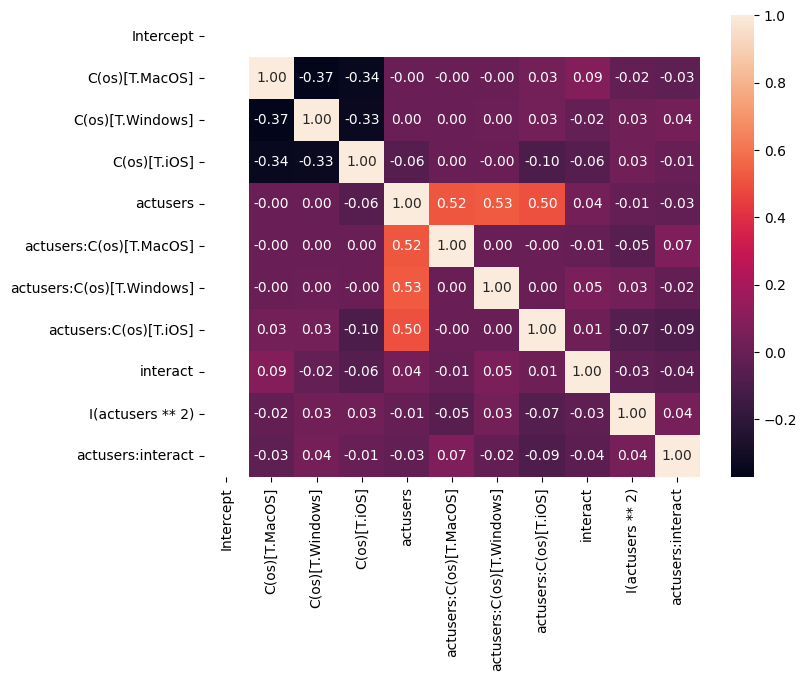
\includegraphics[width=0.8\textwidth]{img/korelace_promennych.png}
    \caption{Korelace proměnných po prvním kole filtrace statisticky nevýznamných a~korelovaných proměnných.}
    \label{fig:korelace_promennych}
\end{figure}
Můžeme vidět relativně silné korelace mezi \texttt{actusers} a~interakcí této proměnné s~typy operačních systémů.
Myšlenkou je, že pomocí všech tří interakcí s~OS se dá dobře odhadnout počet aktivních uživatelů, díky čemuž je proměnná \texttt{actusers} v~modelu zbytečná.
Hodnoty VIF nám to napůl potvrzují, hodnota $\mathord{\approx}4.9$ je dost a~interakce s~OS mají hodnotu nad 2, což také není optimální.
Pojďme tedy proměnnou \texttt{actusers} odstranit a~podívat se, co to udělá s~modelem.

Hodnoty koeficientů determinace $R^2$ a~$R^2_{adj}$ zůstaly úplně stejné, a~to na hodnotě $\mathord{\approx}0.84$.
Dále, F-statistika pro celý model se také nezměnila, zůstala na hodnotě $264.4$, p-hodnota F-statistiky je stále $1.69 \cdot 10^{-190}$.
Log-likelihood zůstal na hodnotě -1599.1, AIC (3220) a~BIC (3267) se také nezměnily.
V~Tabulce~\ref{tab:vif_2} je pak vidět, že všechny VIF hodnoty jsou téměř 1, což indikuje téměř žádnou kolinearitu mezi proměnnými, což jsme přesně chtěli.

\begin{wraptable}{l}{0.4\textwidth}
    \centering
    \begin{tabularx}{0.4\textwidth}{lC}
        \toprule
        \textbf{Proměnná} & \textbf{VIF} \\
        \midrule
        Intercept                & 5.520433 \\
        C(os)[T.MacOS]           & 1.638202 \\
        C(os)[T.Windows]         & 1.626717 \\
        C(os)[T.iOS]             & 1.596451 \\
        interact                 & 1.014742 \\
        I(actusers ** 2)         & 1.018598 \\
        actusers:interact        & 1.019165 \\
        actusers:C(os)[Android]  & 1.017360 \\
        actusers:C(os)[MacOS]    & 1.007737 \\
        actusers:C(os)[Windows]  & 1.004390 \\
        actusers:C(os)[iOS]      & 1.021672 \\
        \bottomrule
    \end{tabularx}
    \caption{VIF hodnoty po odstranění proměnné \texttt{actusers}.}
    \label{tab:vif_2}
    \vspace{-3.3em}
\end{wraptable}

Jen nám přibyl OS Android, který se předtím dal jednoduše spočítat z~aktivních uživatelů a~interakcí s~ostatními OS.
Vzhledem k~jeho velmi nízké kolinearitě s~ostatními proměnnými jej zachováme -- i~logicky to dává smysl, tuto hodnotu bychom z~ostatních proměnných neodhadli.

Finální rovnicí modelu tedy je:
\begin{align*}
    \text{ping} &=\beta_0 + \beta_1 \cdot \text{InteractingPct} \\
    &+ \beta_2 \cdot \text{OSType} + \beta_3 \cdot (\text{ActiveUsers}^2) \\
    &+ \beta_4 \cdot (\text{ActiveUsers} \cdot \text{InteractingPct}) \\
    &+ \beta_5 \cdot (\text{ActiveUsers} \cdot \text{OSType})
\end{align*}
Nyní pro všechny hodnoty modelu platí, že jejich p-hodnota je 0 nebo téměř 0 (ale tak malé číslo, že Python jej bere jako 0).
To znamená, že máme model, ve kterém jsou všechny proměnné statisticky významné.
Zároveň jsme ale dost filtrovali.

Z~hodnot $R^2$, $R^2_{adj}$, $F\mathord{-}stat$ a~její p-hodnoty, které byly zmíněny výše, vyčteme, že model dobře popisuje danou problematiku.
Hodnoty AIC a BIC jsou vyšší, protože model je relativně komplexní, což tyhle hodnoty penalizují.

Kód pro vytvoření modelu a~standardizaci atributů (přejmenování sloupečků nezahrnuto), výpočet VIF koeficientů a~korelační matice:

\begin{minted}{python3}
    df = pd.read_excel("data/Data_2024.xlsx", sheet_name="Data_regrese")
    formula = "ping ~ actusers + interact + C(os)+ I(actusers**2) \
        + actusers:interact + actusers:C(os)"

    model = smf.ols(formula=formula, data=df)
    results = model.fit()

    dfS = df.copy()
    dfS[["actusers", "interact", "scroll"]] = (dfS[["actusers", "interact", "scroll"]] - \ 
        dfS[["actusers", "interact", "scroll"]].mean()) / \ 
        dfS[["actusers", "interact", "scroll"]].std()

    model2 = smf.ols(formula=formula, data=dfS)
    results2 = model2.fit()

    X = pd.DataFrame(model2.exog, columns=model2.exog_names)
    vif = pd.Series([variance_inflation_factor(X.values, i)
                    for i in range(X.shape[1])],
                    index=X.columns)
    df_corr = X.corr()
\end{minted}

Nastal čas na nalezení a~případně vyloučení outlierů.
Než začneme, můžeme se podívat na Durbin-Watsonovu statistiku, která dokáže najít autokorelaci v~reziduích, v~takovém případě máme porušenou podmínku nezávislosti reziduí pro lineární regresi.
Ta je $1.928$, což značí skoro žádnou míru autokorelace.

Nejdříve získáme \emph{leverages} (páky) bodů, standardizovaná rezidua, studentizovaná rezidua a~jejich p-hodnoty, Cookovy vzdálenosti a~jejich p-hodnoty.
Vyfiltrujeme zajímavé hodnoty tak, aby splňovaly alespoň jednu z~následujících podmínek:
\begin{itemize}
    \item Leverage větší než $\frac{3k}{n}$, kde $k$ je počet prediktorů modelu a~$n$ je počet pozorování.
    \item Standardizované reziduum je v~absolutní hodnotě větší než 2.
    \item P-hodnota studentizovaného rezidua je nižší než $0.05$, kde $0.05$ je kvantil studentova t-rozdělení.
\end{itemize} 
Takovýchto hodnot je v~datech 14, nicméně všechny hodnoty kromě dvou se pohybují na přelomu hranice outlier/neoutlier.
Hodnoty těch dvou datových vzorků jsou v~Tabulce~\ref{tab:outliers}.
\begin{table}[ht]
    \centering
    \begin{tabularx}{\textwidth}{lXXXXXX}
        \toprule
        &\textbf{Leverage} & \textbf{Standard Residuals} & \textbf{Student Residuals} & \textbf{Student Residuals p-value} & \textbf{Cook's Distance} & \textbf{Cook's Distance p-value} \\
        \midrule
        255 & 0.0100 & 5.9455 & 6.1655 & 1.4679e-09 & 0.0324 & 1.0000 \\
        476 & 0.0749 & 8.8304 & 9.6182 & 0.0000e+00 & 0.5743 & 0.8501 \\
        \bottomrule
    \end{tabularx}
    \caption{Největší favorité na outliery.}
    \label{tab:outliers}
\end{table}
Pro tato data jsou hodnoty standardizovaných i~studentizovaných reziduí velmi velká, p-hodnota je téměř 0.
Průměrná Cookova vzdálenost se v~datech pohybuje kolem $0.002$ $\implies$ ačkoliv se to nezdá, obě dvě tato pozorování mají velký vliv na model, obzvláště druhé dato.

Nicméně, abychom měli jistotu, že tato data můžeme opravdu považovat za outliery, pojďme si vizualizovat rezidua několika způsoby, a~to pomocí Q-Q grafu, histogramu reziduí a~grafy reziduí vzhledem k~predikovaným hodnotám a~pořadí prvků.
Všechny grafy jsou na Obrázku~\ref{fig:rezidua}.
\begin{figure}[ht]
    \centering
    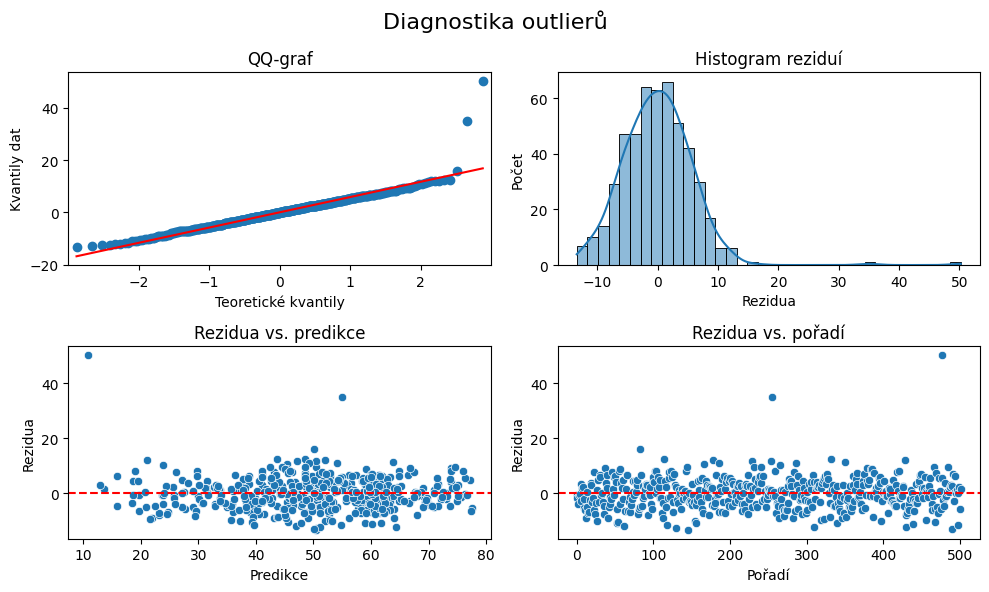
\includegraphics[width=\textwidth]{img/outlier_diagnostics.png}
    \caption{Grafy pro diagnostiku reziduí.}
    \label{fig:rezidua}
\end{figure}

Není třeba se na grafy dívat moc dlouho, abychom zjistili, že v každém grafu figurují dva outliery a~při podrobném pohledu na graf \emph{rezidua vs. pořadí} zjistíme, že jsou zhruba na indexu 250 a~480, tedy korespondují s~našimi favority na outliery.
Mají na model obrovský vliv a~dají se považovat za extrémně odlehlé hodnoty $\implies$~jdou z~dat pryč.

Po odstranění těchto dvou outlierů se vylepšily snad všechny charakteristiky modelu.
Původní hodnoty a~nové hodnoty jsou v~Tabulce~\ref{tab:without_outliers}.
\begin{table}[h!]
    \centering
    \begin{tabularx}{0.7\textwidth}{XRR}
        \toprule
        \textbf{Charakteristika} & \textbf{Stará hodnota} & \textbf{Nová hodnota} \\
        \midrule
        $R^2$ & 0.843 & 0.877 \\
        $R^2_{adj}$ & 0.840 & 0.875 \\
        F-statistika & 264.400 & 349.900 \\
        P(F-stat) & $1.69 \cdot 10^{-190}$ & $1.25 \cdot 10^{-215}$ \\
        Log-likelihood & -1599.100 & -1528.700\\
        AIC & 3220.000 & 3079.000 \\
        BIC & 3267.000 & 3126.000 \\
        Omnibus & 230.750 & 0.661\\
        P(Omnibus) & 0.000 & 0.719\\
        Skew & 1.617 & 0.014\\
        Kurtosis & 15.066 & 2.812\\
        Durbin-Watson & 1.928 & 1.990 \\
        \bottomrule
    \end{tabularx}
    \caption{Změny hodnot charakteristik modelu po vyčištění outlierů.}
    \label{tab:without_outliers}
\end{table}
Všimněme si hlavně obrovského rozdílu ve špičatosti a~šikmosti -- dle \emph{Omnibus} testu rezidua předtím vůbec nebyla normálně rozložena, teď je p-hodnota $\mathord{\approx}0.7$, což je hodně daleko od zamítnutí hypotézy o~normalitě reziduí.
Dá se to i~vyčíst z~konkrétních čísel, normální rozdělení má $SKEW = 0$, $KURT = 3$. 
Velmi dobrá je i~F-statistika a~její p-hodnota.
Log-likelihood, AIC, BIC se zlepšily (ale stále nic moc kvůli složitosti modelu).
Autokorelační Durbin-Watsonův koeficient je, inženýrsky řečeno, $\mathord{\approx}2$.
Díky těmto znalostem můžeme prohlásit, že model opravdu splňuje předpoklady lineární regrese.

Kód k~posledním několika odstavcům (v~podstatě celé recyklováno z~democvičení):
\begin{minted}{python3}
    influence = results2.get_influence()
    leverage = influence.hat_matrix_diag
    cooks_d, cooks_d_pval = influence.cooks_distance
    standardized_residuals = influence.resid_studentized_internal
    studentized_residuals = influence.resid_studentized_external
    studentized_residuals_pvalues = \
        2 * (1 - stats.t.cdf(np.abs(studentized_residuals),
            df=df.shape[0] - len(results2.params)))

    outl_stats_df = pd.DataFrame({
        "Leverage": leverage,
        "Standardized Residuals": standardized_residuals,
        "Studentized Residuals": studentized_residuals,
        "Studentized Residuals p-value": studentized_residuals_pvalues,
        "Cook's Distance": cooks_d,
        "Cook's Distance_p-value": cooks_d_pval
    }, index=df.index)

    print(outl_stats_df["Cook's Distance"].mean())

    outl_stats_df = outl_stats_df[(outl_stats_df["Leverage"] > \
                            3*len(results.params)/df.shape[0]) | \
        (np.abs(outl_stats_df["Standardized Residuals"]) > 2) | \
        (outl_stats_df["Cook's Distance_p-value"] < 0.05)]
\end{minted}

\subsection{Hledání parametrů s největší hodnotou}

Nejjednoduší způsob hledání maxima je dřevorubecká brute-force metoda.
Dala by se určitě použít inteligentnější, nicméně tento model není výpočetně extra náročný, a~proto si to můžeme dovolit.
Navíc to není metoda nějak extra nestandardní.
Kód:
\begin{minted}{python3}
    n_samples = 1000000

    interact_samples = np.random.uniform(
        df["interact"].min(), df["interact"].max(), n_samples)
    actusers_samples = np.random.uniform(
        df["actusers"].min(), df["actusers"].max(), n_samples)
    os_samples = np.random.choice(df["os"].unique(), n_samples)

    sample_data = pd.DataFrame({
        "interact": interact_samples,
        "actusers": actusers_samples,
        "os": os_samples
    })

    sample_data["predicted_ping"] = results.predict(sample_data)

    max_values = sample_data.loc[sample_data["predicted_ping"].idxmax()]
\end{minted}
Pro větší modely, které potřebují více dat, se mohou použít metody jako \emph{Latin hypercube sampling}, které rovnoměrně vyplní prostor.
Nám stačí náhodně vygenerovat milion vzorků náhodných dat a~ty pokryjí velkou část domény, na které pracujeme.
Po několika spuštěních vycházely stále podobné hodnoty.
Zjištěné hodnoty:
\begin{table}[h!]
    \centering
    \begin{tabularx}{0.4\textwidth}{|X|R|}
        \hline
        ping & 77.589 \\
        \hline
        interacting & 0.997 \\
        \hline
        active users & 9787.758 \\
        \hline
    \end{tabularx}
\end{table}

\subsection{Odhad pingu, konfidenční a predikční interval}

Pro tuto úlohu stačí vytvořit dataframe o~jednom řádku, jehož hodnoty budou průměry parametrů interaktivity a~aktivních uživatelů, OS bude zvolen Windows dle zadání.
Veškeré informace pro konfidenční, predikční interval a~průměrnou predikovanou hodnotu poskytnou vestavěné funkce modulu \texttt{statsmodel}.
Kód je v~tomto případě velmi jednoduchý.
\begin{minted}{python3}
    prediction_data = pd.DataFrame({
        "interact": [df["interact"].mean()],
        "actusers": [df["actusers"].mean()],
        "os": ["Windows"]
    })

    predictions = results.get_prediction(prediction_data)
    summary_frame = predictions.summary_frame(alpha=0.05)
\end{minted}
\texttt{summary\textunderscore frame} je dataframe, stačí z~něj extrahovat hodnoty, které potřebujeme.
Výsledek:
\begin{table}[ht]
    \centering
    \begin{tabularx}{0.5\textwidth}{|X|C|}
        \hline
        Průměrný ping & 55.003 \\ 
        \hline
        Konfidenční interval & $[53.972, 56.033]$ \\
        \hline
        Predikční interval & $[44.725, 65.281]$\\
        \hline
    \end{tabularx}
\end{table}

\subsection{Je model vhodný pro další použití?}

Co se charakteristik týče, model je kvalitní.
$R^2$ i~$R^2_{adj}$ jsou na pěkných hodnotách, podle F-statistiky je model statisticky významný, všechny prediktory v~osekaném modelu jsou statisticky významné, je téměř nulová autokorelace a~rezidua mají hodně blízko k~normálnímu rozdělení, VIF hodnoty všech atributů v~osekaném modelu se pohybují kolem jedničky a~mezi atributy není téměř žádná korelace. 

Osobně si myslím, že pro malé aplikace podobné jako té z~\uv{příběhu} dat se tento model využít dá, pokud by dávalo smysl použít stejné prediktory.
Za použití stejných prediktorů pro větší aplikaci by to mohlo být problémové vzhledem k tomu, že růst aktivních uživatelů dost ovlivňuje růst odhadované odezvy appky a~po překročení nějakého počtu uživatelů by to predikovalo nesmysly; jinými slovy, myslím si, že je model přetrénován na moc malých oborech hodnot atributů (především tedy počet uživatelů).

\end{document}